\documentclass[universe,article,submit,pdftex,moreauthors]{Definitions/mdpi}
\usepackage{amsmath,amssymb,amsfonts}
\usepackage{graphicx}
\usepackage{physics}
\usepackage{tikz}
\usepackage{amsopn}
\usepackage{amstext}
\usepackage{microtype}
\usepackage{xparse}
\usepackage{algorithm}
\usepackage{algorithmicx}
\usepackage{algpseudocode}
% Boxes
\usepackage[most]{tcolorbox}
% Plots (pgfplots provides axis/addplot)
\usepackage{pgfplots}
\usetikzlibrary{intersections}
\usepgfplotslibrary{fillbetween}
\pgfplotsset{compat=1.18}
\NewDocumentCommand{\subsubsubsection}{s m}{%
  \IfBooleanTF{#1}{\paragraph*{#2}}{\paragraph{#2}}%
}
\usetikzlibrary
{arrows.meta, calc, fit, decorations.pathmorphing, decorations.pathreplacing, shapes.geometric, shadings, positioning,
  decorations.markings, patterns}
\theoremstyle{remark}
\newtheorem*{remark}{Remark}
\theoremstyle{definition}

\firstpage{1}
\setcounter{page}{\@firstpage}
\pubvolume{1}
\issuenum{1}
\articlenumber{0}
\pubyear{2026}
\copyrightyear{2026}
\datereceived{ }
\daterevised{ } % Comment out if no revised date
\dateaccepted{ }
\datepublished{ }
\doinum{}

\Title{A Single Effective Framework Underlying Galaxy Rotation Curves and the Hubble Tension}

\newcommand{\orcidauthorA}{0009-0001-7697-7868}

\Author{Jerome Beau$^{1,*}$}

\AuthorNames{Jerome Beau}

\address{%
  \quad Independent Researcher, France; jerome.beau@cosmochrony.org}

\corres{Correspondence: jerome.beau@cosmochrony.org}

\abstract
{We investigate whether two long-standing observational anomalies---flat galaxy rotation curves and the Hubble constant
tension---may originate from a common effective mechanism operating in low-density environments. We introduce a minimal
phenomenological framework in which departures from Newtonian expectations arise from a bounded saturation of the
effective gravitational response at the level of kinematic inference,
  without invoking dark matter particles or modifying the background Friedmann expansion or early-universe physics. In
  the galactic regime,
  the empirically established low-acceleration phenomenology arises as the saturated limit of the effective kinematic
  inference,
  with no modification of the gravitational law. Applied to disk galaxies,
  the framework reproduces the main features of observed rotation curves across a broad range of morphologies using
  baryonic matter alone,
  with stable parameter values and no halo-by-halo tuning; comparisons with representative galaxies from the SPARC
  sample show that the effective saturation scale correlates with observed surface-density-dependent trends. At
  cosmological scales,
  the same bounded-response structure predicts environment-dependent shifts in the locally inferred expansion rate:
  for typical void density contrasts the deep-saturation regime applies,
  yielding a fractional shift $\Delta H/H \simeq \delta_\rho f_{\max}$
  without additional cosmological degrees of freedom or any change to the global expansion history. We examine
  robustness, degeneracies, and limitations,
  and outline distinctive observational signatures,
  including environment-dependent redshift drift and weak-lensing modifications in extreme low-acceleration regimes.
  We finally isolate a structural expansion sector: under an explicitly stated rank--time dictionary hypothesis,
  the accelerated component of expansion is carried by the branching of projectively distinguishable histories---an
  exact Pell count with rate $\log(1+\sqrt{2})$---rather than by a dark-energy fluid,
  the naive state-volume reading is quantitatively excluded,
  and the asymptotic de Sitter limit is upgraded from a free late-time fit to a calibrated spectral steady state,
  with no numerical prediction of $H_\infty$. Interpretive reading (interpretation, not a derived result): the
  late-time anomalies trace inference bounds rather than new substances,
  and accelerated expansion is a property of the projective record.}

\keyword{cosmology; galaxy rotation curves; Hubble tension; galactic dynamics; voids}

\providecommand{\bibcommenthead}{}

\begin{document}

  \input{01-introduction/introduction}
  \input{02-effective_model/effective_model}
  \section{Galaxy Rotation Curves}
  \label{sec:rotation_curves}

  We now test the effective model introduced in
  Section~\ref{sec:effective_model} against observed galaxy rotation curves.
  The goal of this section is not to achieve maximal fitting flexibility, but to
  assess whether a single effective saturation scale can reproduce the main
  kinematic features of disk galaxies using baryonic matter alone.

  A useful internal consistency requirement is that the acceleration scale
  governing the transition be determined directly from galactic kinematic data.
  For the SPARC sample, fitting the effective model to the observed rotation
  curves yields a characteristic transition scale of order
  $10^{-10}\,\mathrm{m\,s^{-2}}$.
  This value is obtained within the present framework solely from galaxy
  rotation data and does not rely on any cosmological prior or assumption
  regarding the Hubble constant.

  The numerical value is consistent with the empirical acceleration scale
  previously identified in the MOND literature~\cite{McGaugh2016}.
  Here, however, this scale is interpreted as the onset of a bounded-response
  regime in the effective description, rather than as a fundamental constant
  modifying the gravitational law.

  This motivates treating $a_\star$ as a single universal effective scale
  consistently appearing in both high- and low-surface-density galaxies,
  without requiring modifications to early-time cosmology or additional
  dark components.

  \subsection{Data and Methodology}
  \label{subsec:data_method}

  We use the SPARC database, which provides high-quality rotation curves together
  with homogeneous photometry and baryonic mass models for disk galaxies spanning
  a wide range of morphologies, surface brightnesses, and dynamical regimes~\cite{Lelli2016SPARC}.

  The numerical pipeline used to generate the rotation-curve figures and diagnostics is available as open-source
  software~\cite{CosmochronySimulation}.

  For each galaxy, the baryonic mass distribution is constructed from the observed stellar and gas components.
  Stellar mass-to-light ratios are fixed following the standard SPARC prescriptions.
  No additional dark matter component is introduced in this effective description.

  The effective acceleration $g_{\mathrm{eff}}(r)$ is obtained by solving
  Eq.~\eqref{eq:effective_acceleration} using the Newtonian acceleration
  $g_{\mathrm{N}}(r)$ computed from the baryonic mass distribution.
  The circular velocity then follows from
  \begin{equation}
    v_{\mathrm{eff}}(r) = \sqrt{r\, g_{\mathrm{eff}}(r)} .
  \end{equation}

  The saturation scale $a_\star$ is treated as a universal parameter.
  Its value is fixed globally by minimizing the total residuals across the
  sample, rather than optimized on a galaxy-by-galaxy basis.

  \subsection{Representative Fits}
  \label{subsec:fits}

  We illustrate the performance of the effective model on representative
  galaxies spanning different surface-density regimes.
  The goal is not to emphasize isolated best cases, but to show typical
  behaviors observed across the full SPARC sample.

  High-surface-density galaxies are well described by Newtonian dynamics in
  their inner regions.
  Deviations from Newtonian predictions appear only at large radii, where the
  baryonic acceleration drops below the saturation scale.
  The resulting rotation curves flatten smoothly, without requiring extended
  mass halos, in agreement with observed trends across high-surface-brightness
  disks~\cite{Lelli2016SPARC}.

  Low-surface-brightness galaxies probe the saturated regime over most of their
  radial extent.
  In these systems, the effective acceleration departs from Newtonian behavior
  already at small radii, naturally producing slowly rising and asymptotically
  flat rotation curves, a feature commonly observed in diffuse systems~\cite{McGaugh2016}.

  Across the sample, the model reproduces the observed diversity of rotation
  curve shapes.
  This diversity arises solely from differences in the baryonic mass
  distribution and surface density, not from variations in the effective
  parameters.

  The galaxies shown in Fig.~\ref{fig:rotation-curves} are selected as
  representative well-fitted systems spanning rising, nearly flat,
  and slowly declining rotation curves.
  The saturation scale $a_\star$ is fixed globally from the full-sample
  analysis discussed in Section~\ref{subsec:universality}.
  No galaxy-dependent adjustment of $a_\star$ is performed.

  \begin{figure}
    \centering
    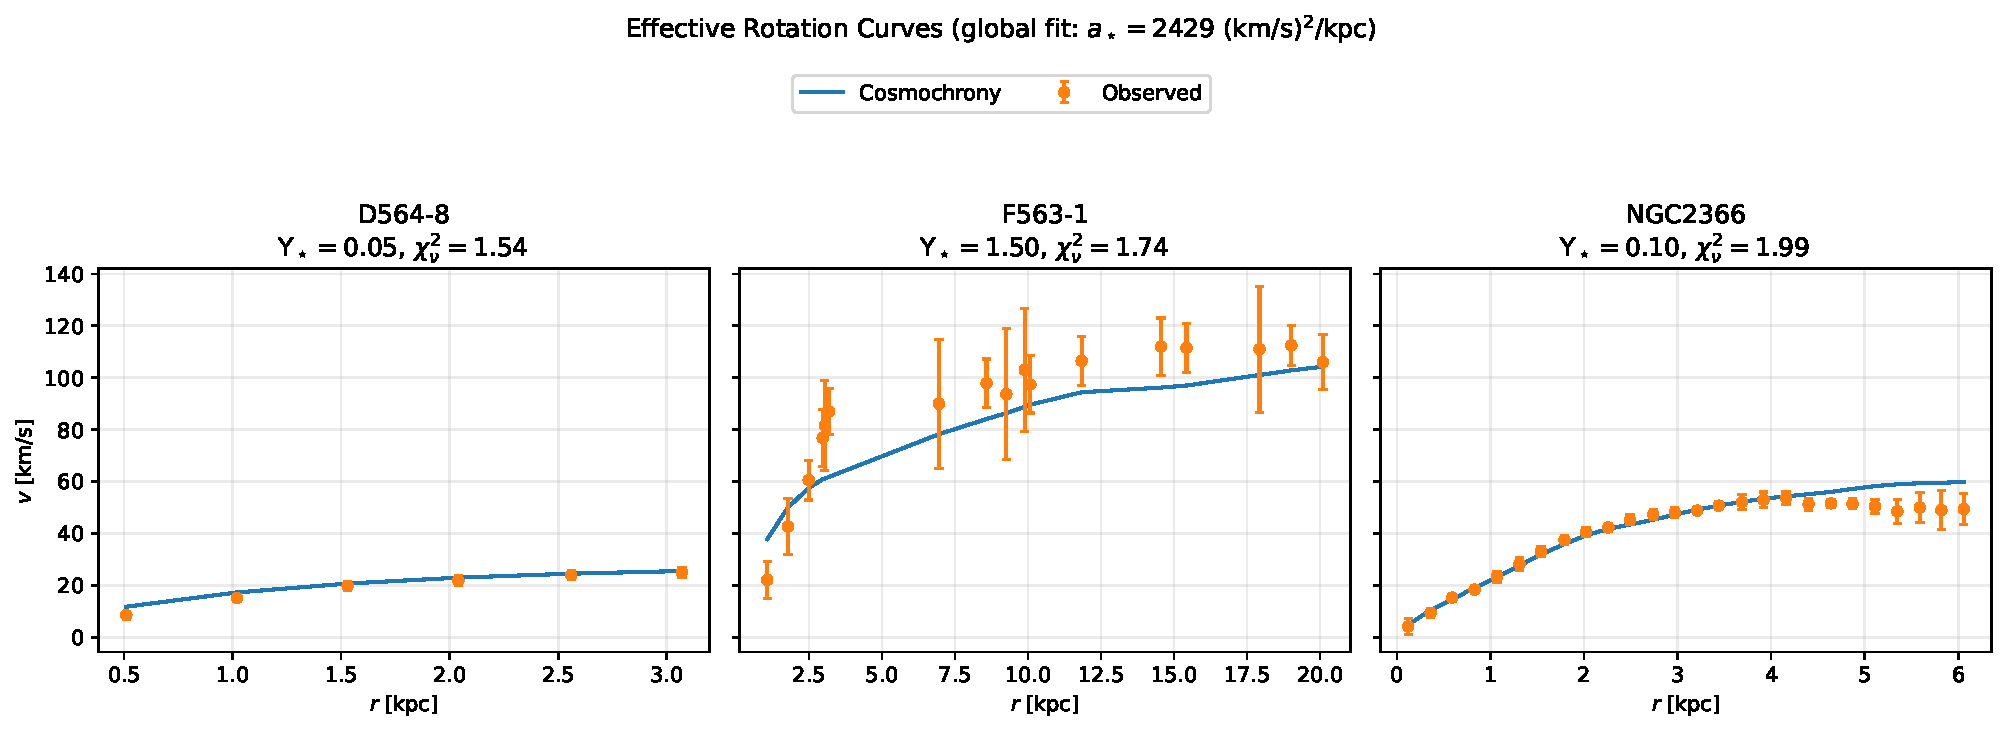
\includegraphics[width=\linewidth]{../code/03-rotation_curves/galaxy_rotcurves_showcase}
    \caption[Representative SPARC rotation curves]{
      Representative galaxy rotation curves from the SPARC sample.
      Observed circular velocities (points) are compared with the effective model
      prediction (solid lines) computed from the baryonic mass distribution alone.
      The three systems span distinct surface-density regimes and kinematic
      behaviors (rising, nearly flat, and mildly declining).
      A single universal saturation scale $a_\star$, determined from the full
      sample, is used for all galaxies.
      The only galaxy-dependent parameter is the stellar mass-to-light ratio
      $\Upsilon_\star$, fitted within a physically motivated interval.
      The code used to generate these curves is publicly available
      \protect\cite{CosmochronySimulation}.
    }
    \label{fig:rotation-curves}
  \end{figure}

  Representative examples illustrating these behaviors are shown in
  Fig.~\ref{fig:rotation-curves}.

  \subsection{Residuals and Scaling Relations}
  \label{subsec:residuals}

  We quantify the quality of the fits using radial velocity residuals
  \begin{equation}
    \Delta v(r) = v_{\mathrm{obs}}(r) - v_{\mathrm{eff}}(r) .
  \end{equation}

  The residuals exhibit no systematic radial trends across the sample.
  In particular, no characteristic scale or radius-dependent bias is observed.

  The effective model naturally reproduces the empirical correlation between
  rotation curve shape and baryonic surface density.
  Galaxies with higher central surface density remain in the Newtonian regime
  over a larger radial range, while diffuse systems enter the saturated regime earlier.

  The transition radius at which rotation curves flatten corresponds closely to
  the regime where the effective surface flux density approaches the saturation limit.
  Beyond this point, further decreases in baryonic density no longer translate
  into stronger dynamical suppression, leading to asymptotically flat rotation velocities.

  This behavior is closely related to the observed radial acceleration relation.
  In the present framework, this relation is not imposed but emerges directly
  from the effective saturation of the gravitational response at low acceleration~\cite{McGaugh2016RAR}.

  \subsection{Universality of the Saturation Scale}
  \label{subsec:universality}

  A key result of the analysis is the stability of the saturation scale $a_\star$ across the sample.
  Allowing moderate variations of $a_\star$ does not significantly improve the
  quality of the fits and tends to introduce degeneracies with baryonic mass normalization.

  This supports the interpretation of $a_\star$ as a universal effective scale
  rather than a phenomenological fitting parameter.
  All galaxy-to-galaxy variability is accounted for by the observed baryonic structure.

  The absence of halo-by-halo tuning distinguishes this approach from standard
  dark matter halo modeling, which typically requires galaxy-dependent halo profiles and parameters.

  The universality of the saturation scale follows from the existence of a
  fundamental bound on the effective flux that can be supported by the geometric substrate.
  Unlike dark matter halo models, the present framework involves a single
  acceleration scale set by an intrinsic saturation of the underlying geometric response.

  \subsection{Summary}
  \label{subsec:rc_summary}

  The effective saturation model reproduces the main phenomenological features
  of galaxy rotation curves across a wide range of systems using baryonic matter alone.
  The same universal saturation scale governs both high- and
  low-surface-density galaxies, with smooth transitions between Newtonian and saturated regimes.

  These results motivate extending the analysis to cosmological low-density environments.
  In the next section, we show that the same effective mechanism leads to
  environment-dependent signatures in the inferred expansion rate, providing a
  natural connection to the Hubble tension.

  The determination of $a_\star$ from galactic rotation curves
  constitutes the only free parameter of the effective model.
  No cosmological quantity, including $H_0$, enters this calibration.
  The cosmological implications discussed in
  Section~\ref{sec:voids_hubble} therefore represent an independent
  consequence of the same empirically fixed scale.


  \input{../code/04-voids_hubble/voids_hubble}
  \input{05-robustness/robustness}
  \section{Expansion as Projective History Branching}
\label{sec:history-branching-expansion}

The preceding sections describe the late-time phenomenological sector of the model.
We now isolate a distinct structural question: whether the accelerated component of cosmic expansion can be
associated with the growth of admissible projective histories rather than with a material dark-energy fluid.

The relevant result is not an exponential growth of Heisenberg balls.
Indeed, the spectral admissibility cascade is carried by the Heisenberg group, whose endpoint balls have
polynomial Bass--Guivarc'h growth of degree four before finite-$q$ saturation.
Endpoint counting therefore cannot support an asymptotic de Sitter-like component.
The surviving exponential object is instead the number of projectively distinguishable
histories~\cite{Beau2026tb}.
For the canonical O12-compatible residual channel, the trajectory-branching note proves that endpoint-based
distinguishability collapses, whereas D4 projective distinguishability yields the exact Pell count
\[
N_{\mathrm{dist}}(n)=N_b(n),
\qquad
N_b(n)=2N_b(n-1)+N_b(n-2),
\]
with asymptotic rate
\[
h_b=\lim_{n\to\infty}\frac{1}{n}\log N_b(n)
=\log(1+\sqrt{2}).
\]
This relocates the exponential component of the two-regime expansion model of the spectral relaxation
paper~\cite{Beau2026a5} from state volume to history branching.

\begin{hypothesis}[H-dict: rank--time dictionary]
\label{hyp:H-dict}
The coarse-grained homogeneous cosmological update identifies one admissible cascade rank with one projective
clock tick of duration $H^{-1}$.
Equivalently,
\[
dt = H^{-1}dn,
\qquad
dn = H\,dt = d\log a.
\]
Thus, up to an additive constant, the cascade rank is the number of e-folds,
\[
n=\log a.
\]
\end{hypothesis}

Hypothesis~\ref{hyp:H-dict} is a dictionary between the temporal-ordering sector and the homogeneous
cosmological sector.
It is not an additional expansion law.
It fixes how the already-defined projective rank is read by the effective FRW observer.
Its two ingredients are already separately established: the temporal-ordering sector identifies one
admissible cascade rank with one intrinsic tick~\cite{Beau2026tp}, and the operational closure of
Appendix~\ref{app:cosmo_resolution} identifies $H^{-1}$ as the unique intrinsic update timescale of the
homogeneous regime.
What Hypothesis~\ref{hyp:H-dict} adds --- and what keeps it a hypothesis rather than a theorem --- is the
identification of the discrete projective rank of the substrate cascade with the coarse-grained homogeneous
update step, a bridge between sub-programmes.

Under Hypothesis~\ref{hyp:H-dict}, the canonical projective history count scales as
\[
N_{\mathrm{dist}}(a)\sim a^{h_b},
\qquad
h_b=\log(1+\sqrt{2})\simeq 0.881.
\]
This immediately rules out the naive volumetric interpretation $N_{\mathrm{dist}}\propto a^3$: the exponent
mismatch ($0.881$ against $3$) makes the identification quantitatively impossible, independently of the
structural endpoint no-go.
The branching count is not the comoving volume of space.
It is the entropy-bearing count of distinguishable reprojection histories.

The de Sitter-like reading is therefore structural.
The accelerated component is not sourced by a material fluid with negative pressure.
It reflects the persistence of a positive projective history-branching rate: the admissible space of future
reprojections does not terminate under the Heisenberg transfer.

Two clarifications protect this statement.
First, under Hypothesis~\ref{hyp:H-dict} the exponential growth in rank is a power law in the scale factor by
construction; the branching result therefore does not by itself determine $H(t)$, and in particular does not
derive the acceleration of the scale factor.
What it establishes is that the projective sector sustains, rather than obstructs, unbounded e-folding, and
that it assigns to the accelerated phase a definite entropy carrier, with history-entropy production rate
$\dot S_{\mathrm{hist}} = h_b\,H$.
Second, the value of the asymptotic Hubble scale $H_\infty$ is not fixed by the Pell rate alone.
It requires the normalization of projective rank against the physical homogeneous clock and is left as an
open normalization problem.
The named corpus route towards such a normalization is the variational principle of the spectral-equilibrium
sector, where the Einstein response arises as an Euler--Lagrange condition of a renormalized spectral
entropy~\cite{Beau2026Thermodynamics}; connecting the history-branching entropy to that variational object is
an open front, not used here.

The canonical channel is rigid and gives a constant branching rate.
A time-dependent effective equation of state, if present, must come from the compression of full-history
profiles rather than from the $b$-shadow channel.
The full-history Gabor channel provides the current candidate for such a compression
profile~\cite{Beau2026tb}, but its canonical cosmological interpretation remains open.

\subsection{Large-angle imprint of the pre-branching regime}
\label{subsec:low-ell-prebranching}

The projective history-branching result also clarifies a possible origin of the low-$\ell$ anomaly discussed
in the earlier white-paper formulation~\cite{Cosmochrony}.
In the canonical D4 channel, the first ranks are projectively degenerate: the number of distinguishable
histories is small before the Pell branching regime becomes effective.
Under Hypothesis~\ref{hyp:H-dict}, the smallest cascade ranks correspond to the largest observable scales.
A suppression of distinguishable projective histories at $n\leq 2$ is therefore a natural candidate mechanism
for a suppression of large-angle variance.

This statement should not be confused with a derivation of the observed low-$\ell$ spectrum.
The earlier ratio $\lambda_2/\lambda_1\simeq 8/3$ belongs to the $S^3$/Hopf spectral relaxation experiments
of the white paper and must be re-audited in the Heisenberg D4 setting.
The present result supplies the missing structural mechanism: a pre-branching window in which projectively
distinguishable histories have not yet reached their asymptotic entropy rate.
The quantitative link to CMB multipoles remains open.

  \input{06-predictions/predictions}
  \input{07-conclusion/conclusion}

  \appendix
  \newcounter{defctr}[section]
\renewcommand{\thedefctr}{\thesection.\arabic{defctr}}

\section{Cosmological Operational Closure and the Scale $\ell = c/H$}
  \label{app:cosmo_resolution}

  This appendix derives Eq.~\eqref{eq:ell_cosmo} used in Section~\ref{subsec:cosmo_resolution}.
  The derivation relies solely on the operational closure axiom and the
  homogeneous saturated kinematics of the projected state.
  No geometric horizon concept is invoked.

  \subsection{A.1 Operational closure and descriptive resolution}
    \label{subsec:operational-closure}

    \refstepcounter{defctr}\label{def:ell_closure}
    \noindent\textbf{Definition~\thedefctr\ (Operational closure and descriptive resolution).}
    The descriptive resolution $\ell$ is the minimal coarse-graining neighbourhood such that the update of the
    projected state $U$ at epoch $t$ depends on all substrate channels that can influence the update within a
    single admissible step, and on no others.
    \par\medskip

    \noindent By definition~\ref{def:ell_closure}, the descriptive resolution $\ell$
    is the minimal coarse-graining neighbourhood such that the update of the
    projected state $U$ at epoch $t$ depends on all substrate channels that can
    influence the update within a single admissible step, and on no others.

    Closure therefore requires two properties:

    \begin{enumerate}
      \item Completeness: all admissible influences must be included.
      \item Minimality: no inadmissible or causally irrelevant regions are included.
    \end{enumerate}

  \subsection{Homogeneous saturated kinematics}
    \label{subsec:homogeneous-saturated-kinematics}

    In the homogeneous late-time regime,
    \begin{equation}
      D_{\mathrm{loc}}\chi_{\mathrm{eff}} = c,
    \end{equation}
    so propagation of relational influence is bounded by $c$.

    The projected state evolves according to
    \begin{equation}
      H(t) = \frac{\dot{\chi}}{\chi}.
    \end{equation}

    In a homogeneous regime, $H(t)$ is the unique intrinsic dimensionless rate.
    The characteristic update time is therefore
    \begin{equation}
      \tau(t) \sim \left(\frac{\dot{\chi}}{\chi}\right)^{-1} = H(t)^{-1}.
    \end{equation}

    This is not imposed externally.
    It follows from the requirement that an update corresponds to an
    order-one change of the dimensionless global state variable.

  \subsection{Influence domain and lower bound}
    \label{subsec:influence-domain-and-lower-bound}

    Within one update step of duration $\tau(t)$, the maximal
    propagation distance of relational influence is
    \begin{equation}
      r_{\mathrm{max}} = c \tau(t) = \frac{c}{H(t)}.
    \end{equation}

    Any substrate configuration at distance $r \le r_{\mathrm{max}}$
    can influence the projected state within the update step.
    Excluding such configurations from the coarse-graining neighbourhood
    would violate completeness of closure.

    Therefore,
    \begin{equation}
      \ell \ge \frac{c}{H(t)}.
    \end{equation}

  \subsection{Minimality and upper bound}
    \label{subsec:minimality-and-upper-bound}

    Conversely, any configuration at distance $r > r_{\mathrm{max}}$
    cannot influence the update within the admissible step.

    Including such regions in the neighbourhood does not modify the update
    map of $U$, but enlarges the coarse-graining domain beyond the minimal
    operationally closed set.

    Minimality of closure therefore requires
    \begin{equation}
      \ell \le \frac{c}{H(t)}.
    \end{equation}

  \subsection{Uniqueness of the homogeneous resolution}
    \label{subsec:uniqueness-of-the-homogeneous-resolution}

    Combining the bounds yields
    \begin{equation}
      \ell_{\mathrm{cosmo}}(t) = \frac{c}{H(t)}.
    \end{equation}

    No additional scale is available in the homogeneous regime.
    Any alternative choice $\ell = f(H)$ would either violate dimensional
    consistency or introduce an extraneous parameter, contradicting
    the ontological minimality of the framework.

  \subsection{Consequence for the saturation scale}
    \label{subsec:consequence-for-the-saturation-scale}

    Substituting into
    \begin{equation}
      a_\star(t) \sim \kappa \frac{c_{\mathrm{BI}}^2}{\ell(t)}
    \end{equation}
    gives
    \begin{equation}
      a_\star(t) \sim \kappa\, \frac{c_{\mathrm{BI}}^2}{c}\, H(t).
    \end{equation}

    In projectable regimes $c_{\mathrm{BI}} \to c$, yielding
    \begin{equation}
      a_\star(t) \sim \kappa\, c H(t).
    \end{equation}

    This establishes a structural link between the galactic
    saturation scale and the cosmological expansion rate.
    The normalization factor $\kappa$ is fixed independently by the
    $\mathrm{U}(1)$ holonomy condition discussed in Section~\ref{subsec:holonomy_normalization}.


  \dataavailability{%
    The galaxy rotation-curve data used in this work are drawn from the publicly available
    SPARC database~\cite{Lelli2016SPARC}.
    The numerical code used to generate the galaxy rotation-curve figures and associated
    diagnostics is openly available and archived with a persistent identifier.
    The version used in this work is available via Zenodo at
    \url{https://doi.org/10.5281/zenodo.18462369}~\cite{CosmochronySimulation}.%
  }

  \acknowledgments
  {The author acknowledges the use of large language models as an editorial and analytical assistant during manuscript
  preparation, including help with phrasing alternatives, consistency checks, and structured rewriting.
  All scientific claims, modelling choices, numerical results, and interpretations are the sole responsibility of the
  author.}

  \conflictsofinterest{The author declares no conflicts of interest.}

  \reftitle{References}
  \bibliography{references}

\end{document}
